% Created by tikzDevice version 0.12.6 on 2025-04-17 10:37:54
% !TEX encoding = UTF-8 Unicode
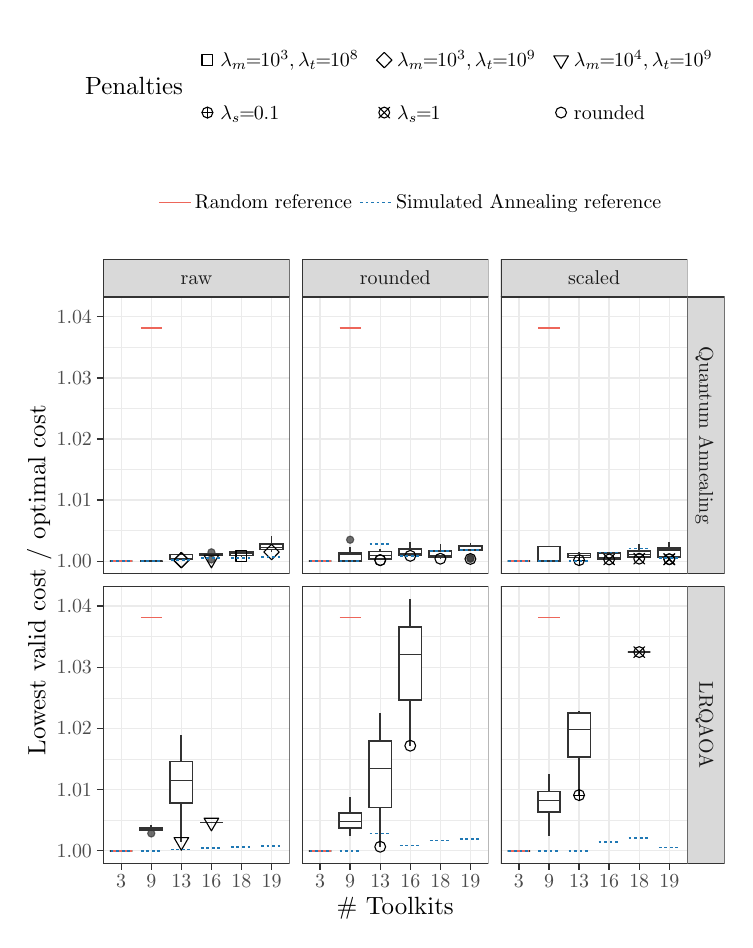
\begin{tikzpicture}[x=1pt,y=1pt]
\definecolor{fillColor}{RGB}{255,255,255}
\path[use as bounding box,fill=fillColor,fill opacity=0.00] (0,0) rectangle (251.81,322.31);
\begin{scope}
\path[clip] (  0.00,  0.00) rectangle (251.81,322.31);
\definecolor{drawColor}{RGB}{255,255,255}
\definecolor{fillColor}{RGB}{255,255,255}

\path[draw=drawColor,line width= 0.5pt,line join=round,line cap=round,fill=fillColor] (  0.00,  0.00) rectangle (251.81,322.31);
\end{scope}
\begin{scope}
\path[clip] ( 27.28,124.93) rectangle ( 94.64,225.00);
\definecolor{fillColor}{RGB}{255,255,255}

\path[fill=fillColor] ( 27.28,124.93) rectangle ( 94.64,225.00);
\definecolor{drawColor}{gray}{0.92}

\path[draw=drawColor,line width= 0.2pt,line join=round] ( 27.28,140.53) --
	( 94.64,140.53);

\path[draw=drawColor,line width= 0.2pt,line join=round] ( 27.28,162.62) --
	( 94.64,162.62);

\path[draw=drawColor,line width= 0.2pt,line join=round] ( 27.28,184.72) --
	( 94.64,184.72);

\path[draw=drawColor,line width= 0.2pt,line join=round] ( 27.28,206.81) --
	( 94.64,206.81);

\path[draw=drawColor,line width= 0.5pt,line join=round] ( 27.28,129.48) --
	( 94.64,129.48);

\path[draw=drawColor,line width= 0.5pt,line join=round] ( 27.28,151.57) --
	( 94.64,151.57);

\path[draw=drawColor,line width= 0.5pt,line join=round] ( 27.28,173.67) --
	( 94.64,173.67);

\path[draw=drawColor,line width= 0.5pt,line join=round] ( 27.28,195.76) --
	( 94.64,195.76);

\path[draw=drawColor,line width= 0.5pt,line join=round] ( 27.28,217.86) --
	( 94.64,217.86);

\path[draw=drawColor,line width= 0.5pt,line join=round] ( 33.80,124.93) --
	( 33.80,225.00);

\path[draw=drawColor,line width= 0.5pt,line join=round] ( 44.66,124.93) --
	( 44.66,225.00);

\path[draw=drawColor,line width= 0.5pt,line join=round] ( 55.52,124.93) --
	( 55.52,225.00);

\path[draw=drawColor,line width= 0.5pt,line join=round] ( 66.39,124.93) --
	( 66.39,225.00);

\path[draw=drawColor,line width= 0.5pt,line join=round] ( 77.25,124.93) --
	( 77.25,225.00);

\path[draw=drawColor,line width= 0.5pt,line join=round] ( 88.12,124.93) --
	( 88.12,225.00);
\definecolor{drawColor}{gray}{0.20}

\path[draw=drawColor,line width= 0.6pt,line join=round] ( 33.80,129.48) -- ( 33.80,129.48);

\path[draw=drawColor,line width= 0.6pt,line join=round] ( 33.80,129.48) -- ( 33.80,129.48);

\path[draw=drawColor,line width= 0.6pt,fill=fillColor] ( 29.72,129.48) --
	( 29.72,129.48) --
	( 37.87,129.48) --
	( 37.87,129.48) --
	( 29.72,129.48) --
	cycle;

\path[draw=drawColor,line width= 0.4pt] ( 29.72,129.48) -- ( 37.87,129.48);

\path[draw=drawColor,line width= 0.6pt,line join=round] ( 44.66,129.48) -- ( 44.66,129.48);

\path[draw=drawColor,line width= 0.6pt,line join=round] ( 44.66,129.48) -- ( 44.66,129.48);

\path[draw=drawColor,line width= 0.6pt,fill=fillColor] ( 40.59,129.48) --
	( 40.59,129.48) --
	( 48.73,129.48) --
	( 48.73,129.48) --
	( 40.59,129.48) --
	cycle;

\path[draw=drawColor,line width= 0.4pt] ( 40.59,129.48) -- ( 48.73,129.48);

\path[draw=drawColor,line width= 0.6pt,line join=round] ( 55.52,131.99) -- ( 55.52,132.98);

\path[draw=drawColor,line width= 0.6pt,line join=round] ( 55.52,130.37) -- ( 55.52,129.90);

\path[draw=drawColor,line width= 0.6pt,fill=fillColor] ( 51.45,131.99) --
	( 51.45,130.37) --
	( 59.60,130.37) --
	( 59.60,131.99) --
	( 51.45,131.99) --
	cycle;

\path[draw=drawColor,line width= 0.4pt] ( 51.45,130.57) -- ( 59.60,130.57);
\definecolor{drawColor}{RGB}{51,51,51}
\definecolor{fillColor}{RGB}{51,51,51}

\path[draw=drawColor,draw opacity=0.70,line width= 0.4pt,line join=round,line cap=round,fill=fillColor,fill opacity=0.70] ( 66.39,130.16) circle (  1.31);

\path[draw=drawColor,draw opacity=0.70,line width= 0.4pt,line join=round,line cap=round,fill=fillColor,fill opacity=0.70] ( 66.39,132.72) circle (  1.31);
\definecolor{drawColor}{gray}{0.20}

\path[draw=drawColor,line width= 0.6pt,line join=round] ( 66.39,132.01) -- ( 66.39,132.17);

\path[draw=drawColor,line width= 0.6pt,line join=round] ( 66.39,131.60) -- ( 66.39,131.13);
\definecolor{fillColor}{RGB}{255,255,255}

\path[draw=drawColor,line width= 0.6pt,fill=fillColor] ( 62.32,132.01) --
	( 62.32,131.60) --
	( 70.46,131.60) --
	( 70.46,132.01) --
	( 62.32,132.01) --
	cycle;

\path[draw=drawColor,line width= 0.4pt] ( 62.32,131.93) -- ( 70.46,131.93);

\path[draw=drawColor,line width= 0.6pt,line join=round] ( 77.25,132.81) -- ( 77.25,133.44);

\path[draw=drawColor,line width= 0.6pt,line join=round] ( 77.25,131.54) -- ( 77.25,131.37);

\path[draw=drawColor,line width= 0.6pt,fill=fillColor] ( 73.18,132.81) --
	( 73.18,131.54) --
	( 81.33,131.54) --
	( 81.33,132.81) --
	( 73.18,132.81) --
	cycle;

\path[draw=drawColor,line width= 0.4pt] ( 73.18,132.42) -- ( 81.33,132.42);

\path[draw=drawColor,line width= 0.6pt,line join=round] ( 88.12,135.82) -- ( 88.12,138.51);

\path[draw=drawColor,line width= 0.6pt,line join=round] ( 88.12,133.80) -- ( 88.12,132.82);

\path[draw=drawColor,line width= 0.6pt,fill=fillColor] ( 84.04,135.82) --
	( 84.04,133.80) --
	( 92.19,133.80) --
	( 92.19,135.82) --
	( 84.04,135.82) --
	cycle;

\path[draw=drawColor,line width= 0.4pt] ( 84.04,134.32) -- ( 92.19,134.32);
\definecolor{drawColor}{RGB}{0,0,0}

\path[draw=drawColor,line width= 0.4pt,line join=round,line cap=round] ( 66.39,127.11) --
	( 69.03,131.69) --
	( 63.75,131.69) --
	cycle;

\path[draw=drawColor,line width= 0.4pt,line join=round,line cap=round] ( 75.29,129.40) rectangle ( 79.22,133.33);

\path[draw=drawColor,line width= 0.4pt,line join=round,line cap=round] ( 52.75,129.90) --
	( 55.52,132.67) --
	( 58.30,129.90) --
	( 55.52,127.12) --
	cycle;

\path[draw=drawColor,line width= 0.4pt,line join=round,line cap=round] ( 52.75,129.90) --
	( 55.52,132.67) --
	( 58.30,129.90) --
	( 55.52,127.12) --
	cycle;

\path[draw=drawColor,line width= 0.4pt,line join=round,line cap=round] ( 85.34,132.82) --
	( 88.12,135.59) --
	( 90.89,132.82) --
	( 88.12,130.04) --
	cycle;
\definecolor{drawColor}{RGB}{237,102,90}

\path[draw=drawColor,line width= 0.6pt,line join=round] ( 29.99,129.48) -- ( 37.60,129.48);

\path[draw=drawColor,line width= 0.6pt,line join=round] ( 40.86,213.78) -- ( 48.46,213.78);
\definecolor{drawColor}{RGB}{31,120,180}

\path[draw=drawColor,line width= 0.6pt,dash pattern=on 1pt off 1pt ,line join=round] ( 40.86,129.48) -- ( 48.46,129.48);

\path[draw=drawColor,line width= 0.6pt,dash pattern=on 1pt off 1pt ,line join=round] ( 73.45,130.76) -- ( 81.06,130.76);

\path[draw=drawColor,line width= 0.6pt,dash pattern=on 1pt off 1pt ,line join=round] ( 51.72,129.90) -- ( 59.33,129.90);

\path[draw=drawColor,line width= 0.6pt,dash pattern=on 1pt off 1pt ,line join=round] ( 29.99,129.48) -- ( 37.60,129.48);

\path[draw=drawColor,line width= 0.6pt,dash pattern=on 1pt off 1pt ,line join=round] ( 84.32,131.15) -- ( 91.92,131.15);

\path[draw=drawColor,line width= 0.6pt,dash pattern=on 1pt off 1pt ,line join=round] ( 62.59,130.58) -- ( 70.19,130.58);
\definecolor{drawColor}{gray}{0.20}

\path[draw=drawColor,line width= 0.5pt,line join=round,line cap=round] ( 27.28,124.93) rectangle ( 94.64,225.00);
\end{scope}
\begin{scope}
\path[clip] ( 27.28, 20.35) rectangle ( 94.64,120.43);
\definecolor{fillColor}{RGB}{255,255,255}

\path[fill=fillColor] ( 27.28, 20.35) rectangle ( 94.64,120.43);
\definecolor{drawColor}{gray}{0.92}

\path[draw=drawColor,line width= 0.2pt,line join=round] ( 27.28, 35.95) --
	( 94.64, 35.95);

\path[draw=drawColor,line width= 0.2pt,line join=round] ( 27.28, 58.04) --
	( 94.64, 58.04);

\path[draw=drawColor,line width= 0.2pt,line join=round] ( 27.28, 80.14) --
	( 94.64, 80.14);

\path[draw=drawColor,line width= 0.2pt,line join=round] ( 27.28,102.23) --
	( 94.64,102.23);

\path[draw=drawColor,line width= 0.5pt,line join=round] ( 27.28, 24.90) --
	( 94.64, 24.90);

\path[draw=drawColor,line width= 0.5pt,line join=round] ( 27.28, 47.00) --
	( 94.64, 47.00);

\path[draw=drawColor,line width= 0.5pt,line join=round] ( 27.28, 69.09) --
	( 94.64, 69.09);

\path[draw=drawColor,line width= 0.5pt,line join=round] ( 27.28, 91.19) --
	( 94.64, 91.19);

\path[draw=drawColor,line width= 0.5pt,line join=round] ( 27.28,113.28) --
	( 94.64,113.28);

\path[draw=drawColor,line width= 0.5pt,line join=round] ( 33.80, 20.35) --
	( 33.80,120.43);

\path[draw=drawColor,line width= 0.5pt,line join=round] ( 44.66, 20.35) --
	( 44.66,120.43);

\path[draw=drawColor,line width= 0.5pt,line join=round] ( 55.52, 20.35) --
	( 55.52,120.43);

\path[draw=drawColor,line width= 0.5pt,line join=round] ( 66.39, 20.35) --
	( 66.39,120.43);

\path[draw=drawColor,line width= 0.5pt,line join=round] ( 77.25, 20.35) --
	( 77.25,120.43);

\path[draw=drawColor,line width= 0.5pt,line join=round] ( 88.12, 20.35) --
	( 88.12,120.43);
\definecolor{drawColor}{gray}{0.20}

\path[draw=drawColor,line width= 0.6pt,line join=round] ( 33.80, 24.90) -- ( 33.80, 24.90);

\path[draw=drawColor,line width= 0.6pt,line join=round] ( 33.80, 24.90) -- ( 33.80, 24.90);

\path[draw=drawColor,line width= 0.6pt,fill=fillColor] ( 29.72, 24.90) --
	( 29.72, 24.90) --
	( 37.87, 24.90) --
	( 37.87, 24.90) --
	( 29.72, 24.90) --
	cycle;

\path[draw=drawColor,line width= 0.4pt] ( 29.72, 24.90) -- ( 37.87, 24.90);
\definecolor{drawColor}{RGB}{51,51,51}
\definecolor{fillColor}{RGB}{51,51,51}

\path[draw=drawColor,draw opacity=0.70,line width= 0.4pt,line join=round,line cap=round,fill=fillColor,fill opacity=0.70] ( 44.66, 31.16) circle (  1.31);
\definecolor{drawColor}{gray}{0.20}

\path[draw=drawColor,line width= 0.6pt,line join=round] ( 44.66, 33.08) -- ( 44.66, 34.21);

\path[draw=drawColor,line width= 0.6pt,line join=round] ( 44.66, 32.32) -- ( 44.66, 32.32);
\definecolor{fillColor}{RGB}{255,255,255}

\path[draw=drawColor,line width= 0.6pt,fill=fillColor] ( 40.59, 33.08) --
	( 40.59, 32.32) --
	( 48.73, 32.32) --
	( 48.73, 33.08) --
	( 40.59, 33.08) --
	cycle;

\path[draw=drawColor,line width= 0.4pt] ( 40.59, 32.70) -- ( 48.73, 32.70);

\path[draw=drawColor,line width= 0.6pt,line join=round] ( 55.52, 57.10) -- ( 55.52, 66.61);

\path[draw=drawColor,line width= 0.6pt,line join=round] ( 55.52, 42.19) -- ( 55.52, 28.13);

\path[draw=drawColor,line width= 0.6pt,fill=fillColor] ( 51.45, 57.10) --
	( 51.45, 42.19) --
	( 59.60, 42.19) --
	( 59.60, 57.10) --
	( 51.45, 57.10) --
	cycle;

\path[draw=drawColor,line width= 0.4pt] ( 51.45, 50.41) -- ( 59.60, 50.41);

\path[draw=drawColor,line width= 0.6pt,line join=round] ( 66.39, 35.12) -- ( 66.39, 35.12);

\path[draw=drawColor,line width= 0.6pt,line join=round] ( 66.39, 35.12) -- ( 66.39, 35.12);

\path[draw=drawColor,line width= 0.6pt,fill=fillColor] ( 62.32, 35.12) --
	( 62.32, 35.12) --
	( 70.46, 35.12) --
	( 70.46, 35.12) --
	( 62.32, 35.12) --
	cycle;

\path[draw=drawColor,line width= 0.4pt] ( 62.32, 35.12) -- ( 70.46, 35.12);
\definecolor{drawColor}{RGB}{0,0,0}

\path[draw=drawColor,line width= 0.4pt,line join=round,line cap=round] ( 55.52, 25.08) --
	( 58.17, 29.65) --
	( 52.88, 29.65) --
	cycle;

\path[draw=drawColor,line width= 0.4pt,line join=round,line cap=round] ( 66.39, 32.07) --
	( 69.03, 36.65) --
	( 63.75, 36.65) --
	cycle;
\definecolor{drawColor}{RGB}{237,102,90}

\path[draw=drawColor,line width= 0.6pt,line join=round] ( 29.99, 24.90) -- ( 37.60, 24.90);

\path[draw=drawColor,line width= 0.6pt,line join=round] ( 40.86,109.20) -- ( 48.46,109.20);
\definecolor{drawColor}{RGB}{31,120,180}

\path[draw=drawColor,line width= 0.6pt,dash pattern=on 1pt off 1pt ,line join=round] ( 40.86, 24.90) -- ( 48.46, 24.90);

\path[draw=drawColor,line width= 0.6pt,dash pattern=on 1pt off 1pt ,line join=round] ( 73.45, 26.19) -- ( 81.06, 26.19);

\path[draw=drawColor,line width= 0.6pt,dash pattern=on 1pt off 1pt ,line join=round] ( 51.72, 25.32) -- ( 59.33, 25.32);

\path[draw=drawColor,line width= 0.6pt,dash pattern=on 1pt off 1pt ,line join=round] ( 29.99, 24.90) -- ( 37.60, 24.90);

\path[draw=drawColor,line width= 0.6pt,dash pattern=on 1pt off 1pt ,line join=round] ( 84.32, 26.58) -- ( 91.92, 26.58);

\path[draw=drawColor,line width= 0.6pt,dash pattern=on 1pt off 1pt ,line join=round] ( 62.59, 26.00) -- ( 70.19, 26.00);
\definecolor{drawColor}{gray}{0.20}

\path[draw=drawColor,line width= 0.5pt,line join=round,line cap=round] ( 27.28, 20.35) rectangle ( 94.64,120.43);
\end{scope}
\begin{scope}
\path[clip] ( 99.14,124.93) rectangle (166.50,225.00);
\definecolor{fillColor}{RGB}{255,255,255}

\path[fill=fillColor] ( 99.14,124.93) rectangle (166.50,225.00);
\definecolor{drawColor}{gray}{0.92}

\path[draw=drawColor,line width= 0.2pt,line join=round] ( 99.14,140.53) --
	(166.50,140.53);

\path[draw=drawColor,line width= 0.2pt,line join=round] ( 99.14,162.62) --
	(166.50,162.62);

\path[draw=drawColor,line width= 0.2pt,line join=round] ( 99.14,184.72) --
	(166.50,184.72);

\path[draw=drawColor,line width= 0.2pt,line join=round] ( 99.14,206.81) --
	(166.50,206.81);

\path[draw=drawColor,line width= 0.5pt,line join=round] ( 99.14,129.48) --
	(166.50,129.48);

\path[draw=drawColor,line width= 0.5pt,line join=round] ( 99.14,151.57) --
	(166.50,151.57);

\path[draw=drawColor,line width= 0.5pt,line join=round] ( 99.14,173.67) --
	(166.50,173.67);

\path[draw=drawColor,line width= 0.5pt,line join=round] ( 99.14,195.76) --
	(166.50,195.76);

\path[draw=drawColor,line width= 0.5pt,line join=round] ( 99.14,217.86) --
	(166.50,217.86);

\path[draw=drawColor,line width= 0.5pt,line join=round] (105.66,124.93) --
	(105.66,225.00);

\path[draw=drawColor,line width= 0.5pt,line join=round] (116.52,124.93) --
	(116.52,225.00);

\path[draw=drawColor,line width= 0.5pt,line join=round] (127.39,124.93) --
	(127.39,225.00);

\path[draw=drawColor,line width= 0.5pt,line join=round] (138.25,124.93) --
	(138.25,225.00);

\path[draw=drawColor,line width= 0.5pt,line join=round] (149.12,124.93) --
	(149.12,225.00);

\path[draw=drawColor,line width= 0.5pt,line join=round] (159.98,124.93) --
	(159.98,225.00);
\definecolor{drawColor}{gray}{0.20}

\path[draw=drawColor,line width= 0.6pt,line join=round] (105.66,129.48) -- (105.66,129.48);

\path[draw=drawColor,line width= 0.6pt,line join=round] (105.66,129.48) -- (105.66,129.48);

\path[draw=drawColor,line width= 0.6pt,fill=fillColor] (101.58,129.48) --
	(101.58,129.48) --
	(109.73,129.48) --
	(109.73,129.48) --
	(101.58,129.48) --
	cycle;

\path[draw=drawColor,line width= 0.4pt] (101.58,129.48) -- (109.73,129.48);
\definecolor{drawColor}{RGB}{51,51,51}
\definecolor{fillColor}{RGB}{51,51,51}

\path[draw=drawColor,draw opacity=0.70,line width= 0.4pt,line join=round,line cap=round,fill=fillColor,fill opacity=0.70] (116.52,137.28) circle (  1.31);
\definecolor{drawColor}{gray}{0.20}

\path[draw=drawColor,line width= 0.6pt,line join=round] (116.52,132.56) -- (116.52,134.80);

\path[draw=drawColor,line width= 0.6pt,line join=round] (116.52,129.48) -- (116.52,129.48);
\definecolor{fillColor}{RGB}{255,255,255}

\path[draw=drawColor,line width= 0.6pt,fill=fillColor] (112.45,132.56) --
	(112.45,129.48) --
	(120.60,129.48) --
	(120.60,132.56) --
	(112.45,132.56) --
	cycle;

\path[draw=drawColor,line width= 0.4pt] (112.45,131.82) -- (120.60,131.82);

\path[draw=drawColor,line width= 0.6pt,line join=round] (127.39,133.04) -- (127.39,133.83);

\path[draw=drawColor,line width= 0.6pt,line join=round] (127.39,130.37) -- (127.39,129.90);

\path[draw=drawColor,line width= 0.6pt,fill=fillColor] (123.31,133.04) --
	(123.31,130.37) --
	(131.46,130.37) --
	(131.46,133.04) --
	(123.31,133.04) --
	cycle;

\path[draw=drawColor,line width= 0.4pt] (123.31,131.60) -- (131.46,131.60);

\path[draw=drawColor,line width= 0.6pt,line join=round] (138.25,133.81) -- (138.25,136.54);

\path[draw=drawColor,line width= 0.6pt,line join=round] (138.25,131.77) -- (138.25,131.45);

\path[draw=drawColor,line width= 0.6pt,fill=fillColor] (134.18,133.81) --
	(134.18,131.77) --
	(142.33,131.77) --
	(142.33,133.81) --
	(134.18,133.81) --
	cycle;

\path[draw=drawColor,line width= 0.4pt] (134.18,132.13) -- (142.33,132.13);

\path[draw=drawColor,line width= 0.6pt,line join=round] (149.12,133.25) -- (149.12,135.73);

\path[draw=drawColor,line width= 0.6pt,line join=round] (149.12,131.11) -- (149.12,130.41);

\path[draw=drawColor,line width= 0.6pt,fill=fillColor] (145.04,133.25) --
	(145.04,131.11) --
	(153.19,131.11) --
	(153.19,133.25) --
	(145.04,133.25) --
	cycle;

\path[draw=drawColor,line width= 0.4pt] (145.04,131.48) -- (153.19,131.48);
\definecolor{drawColor}{RGB}{51,51,51}
\definecolor{fillColor}{RGB}{51,51,51}

\path[draw=drawColor,draw opacity=0.70,line width= 0.4pt,line join=round,line cap=round,fill=fillColor,fill opacity=0.70] (159.98,130.33) circle (  1.31);

\path[draw=drawColor,draw opacity=0.70,line width= 0.4pt,line join=round,line cap=round,fill=fillColor,fill opacity=0.70] (159.98,130.63) circle (  1.31);
\definecolor{drawColor}{gray}{0.20}

\path[draw=drawColor,line width= 0.6pt,line join=round] (159.98,135.07) -- (159.98,136.17);

\path[draw=drawColor,line width= 0.6pt,line join=round] (159.98,133.48) -- (159.98,133.48);
\definecolor{fillColor}{RGB}{255,255,255}

\path[draw=drawColor,line width= 0.6pt,fill=fillColor] (155.91,135.07) --
	(155.91,133.48) --
	(164.05,133.48) --
	(164.05,135.07) --
	(155.91,135.07) --
	cycle;

\path[draw=drawColor,line width= 0.4pt] (155.91,134.75) -- (164.05,134.75);
\definecolor{drawColor}{RGB}{0,0,0}

\path[draw=drawColor,line width= 0.4pt,line join=round,line cap=round] (127.39,129.90) circle (  1.96);

\path[draw=drawColor,line width= 0.4pt,line join=round,line cap=round] (159.98,130.33) circle (  1.96);

\path[draw=drawColor,line width= 0.4pt,line join=round,line cap=round] (138.25,131.45) circle (  1.96);

\path[draw=drawColor,line width= 0.4pt,line join=round,line cap=round] (149.12,130.41) circle (  1.96);

\path[draw=drawColor,line width= 0.4pt,line join=round,line cap=round] (127.39,129.90) circle (  1.96);
\definecolor{drawColor}{RGB}{237,102,90}

\path[draw=drawColor,line width= 0.6pt,line join=round] (112.72,213.78) -- (120.32,213.78);

\path[draw=drawColor,line width= 0.6pt,line join=round] (101.85,129.48) -- (109.46,129.48);
\definecolor{drawColor}{RGB}{31,120,180}

\path[draw=drawColor,line width= 0.6pt,dash pattern=on 1pt off 1pt ,line join=round] (112.72,129.48) -- (120.32,129.48);

\path[draw=drawColor,line width= 0.6pt,dash pattern=on 1pt off 1pt ,line join=round] (134.45,131.32) -- (142.05,131.32);

\path[draw=drawColor,line width= 0.6pt,dash pattern=on 1pt off 1pt ,line join=round] (156.18,133.61) -- (163.78,133.61);

\path[draw=drawColor,line width= 0.6pt,dash pattern=on 1pt off 1pt ,line join=round] (101.85,129.48) -- (109.46,129.48);

\path[draw=drawColor,line width= 0.6pt,dash pattern=on 1pt off 1pt ,line join=round] (145.31,133.13) -- (152.92,133.13);

\path[draw=drawColor,line width= 0.6pt,dash pattern=on 1pt off 1pt ,line join=round] (123.58,135.68) -- (131.19,135.68);
\definecolor{drawColor}{gray}{0.20}

\path[draw=drawColor,line width= 0.5pt,line join=round,line cap=round] ( 99.14,124.93) rectangle (166.50,225.00);
\end{scope}
\begin{scope}
\path[clip] ( 99.14, 20.35) rectangle (166.50,120.43);
\definecolor{fillColor}{RGB}{255,255,255}

\path[fill=fillColor] ( 99.14, 20.35) rectangle (166.50,120.43);
\definecolor{drawColor}{gray}{0.92}

\path[draw=drawColor,line width= 0.2pt,line join=round] ( 99.14, 35.95) --
	(166.50, 35.95);

\path[draw=drawColor,line width= 0.2pt,line join=round] ( 99.14, 58.04) --
	(166.50, 58.04);

\path[draw=drawColor,line width= 0.2pt,line join=round] ( 99.14, 80.14) --
	(166.50, 80.14);

\path[draw=drawColor,line width= 0.2pt,line join=round] ( 99.14,102.23) --
	(166.50,102.23);

\path[draw=drawColor,line width= 0.5pt,line join=round] ( 99.14, 24.90) --
	(166.50, 24.90);

\path[draw=drawColor,line width= 0.5pt,line join=round] ( 99.14, 47.00) --
	(166.50, 47.00);

\path[draw=drawColor,line width= 0.5pt,line join=round] ( 99.14, 69.09) --
	(166.50, 69.09);

\path[draw=drawColor,line width= 0.5pt,line join=round] ( 99.14, 91.19) --
	(166.50, 91.19);

\path[draw=drawColor,line width= 0.5pt,line join=round] ( 99.14,113.28) --
	(166.50,113.28);

\path[draw=drawColor,line width= 0.5pt,line join=round] (105.66, 20.35) --
	(105.66,120.43);

\path[draw=drawColor,line width= 0.5pt,line join=round] (116.52, 20.35) --
	(116.52,120.43);

\path[draw=drawColor,line width= 0.5pt,line join=round] (127.39, 20.35) --
	(127.39,120.43);

\path[draw=drawColor,line width= 0.5pt,line join=round] (138.25, 20.35) --
	(138.25,120.43);

\path[draw=drawColor,line width= 0.5pt,line join=round] (149.12, 20.35) --
	(149.12,120.43);

\path[draw=drawColor,line width= 0.5pt,line join=round] (159.98, 20.35) --
	(159.98,120.43);
\definecolor{drawColor}{gray}{0.20}

\path[draw=drawColor,line width= 0.6pt,line join=round] (105.66, 24.90) -- (105.66, 24.90);

\path[draw=drawColor,line width= 0.6pt,line join=round] (105.66, 24.90) -- (105.66, 24.90);

\path[draw=drawColor,line width= 0.6pt,fill=fillColor] (101.58, 24.90) --
	(101.58, 24.90) --
	(109.73, 24.90) --
	(109.73, 24.90) --
	(101.58, 24.90) --
	cycle;

\path[draw=drawColor,line width= 0.4pt] (101.58, 24.90) -- (109.73, 24.90);

\path[draw=drawColor,line width= 0.6pt,line join=round] (116.52, 38.46) -- (116.52, 44.21);

\path[draw=drawColor,line width= 0.6pt,line join=round] (116.52, 33.21) -- (116.52, 30.22);

\path[draw=drawColor,line width= 0.6pt,fill=fillColor] (112.45, 38.46) --
	(112.45, 33.21) --
	(120.60, 33.21) --
	(120.60, 38.46) --
	(112.45, 38.46) --
	cycle;

\path[draw=drawColor,line width= 0.4pt] (112.45, 35.38) -- (120.60, 35.38);

\path[draw=drawColor,line width= 0.6pt,line join=round] (127.39, 64.64) -- (127.39, 74.61);

\path[draw=drawColor,line width= 0.6pt,line join=round] (127.39, 40.50) -- (127.39, 26.33);

\path[draw=drawColor,line width= 0.6pt,fill=fillColor] (123.31, 64.64) --
	(123.31, 40.50) --
	(131.46, 40.50) --
	(131.46, 64.64) --
	(123.31, 64.64) --
	cycle;

\path[draw=drawColor,line width= 0.4pt] (123.31, 54.67) -- (131.46, 54.67);

\path[draw=drawColor,line width= 0.6pt,line join=round] (138.25,105.76) -- (138.25,115.88);

\path[draw=drawColor,line width= 0.6pt,line join=round] (138.25, 79.25) -- (138.25, 62.84);

\path[draw=drawColor,line width= 0.6pt,fill=fillColor] (134.18,105.76) --
	(134.18, 79.25) --
	(142.33, 79.25) --
	(142.33,105.76) --
	(134.18,105.76) --
	cycle;

\path[draw=drawColor,line width= 0.4pt] (134.18, 95.65) -- (142.33, 95.65);
\definecolor{drawColor}{RGB}{0,0,0}

\path[draw=drawColor,line width= 0.4pt,line join=round,line cap=round] (138.25, 62.84) circle (  1.96);

\path[draw=drawColor,line width= 0.4pt,line join=round,line cap=round] (127.39, 26.33) circle (  1.96);
\definecolor{drawColor}{RGB}{237,102,90}

\path[draw=drawColor,line width= 0.6pt,line join=round] (112.72,109.20) -- (120.32,109.20);

\path[draw=drawColor,line width= 0.6pt,line join=round] (101.85, 24.90) -- (109.46, 24.90);
\definecolor{drawColor}{RGB}{31,120,180}

\path[draw=drawColor,line width= 0.6pt,dash pattern=on 1pt off 1pt ,line join=round] (112.72, 24.90) -- (120.32, 24.90);

\path[draw=drawColor,line width= 0.6pt,dash pattern=on 1pt off 1pt ,line join=round] (134.45, 26.75) -- (142.05, 26.75);

\path[draw=drawColor,line width= 0.6pt,dash pattern=on 1pt off 1pt ,line join=round] (156.18, 29.04) -- (163.78, 29.04);

\path[draw=drawColor,line width= 0.6pt,dash pattern=on 1pt off 1pt ,line join=round] (101.85, 24.90) -- (109.46, 24.90);

\path[draw=drawColor,line width= 0.6pt,dash pattern=on 1pt off 1pt ,line join=round] (145.31, 28.55) -- (152.92, 28.55);

\path[draw=drawColor,line width= 0.6pt,dash pattern=on 1pt off 1pt ,line join=round] (123.58, 31.10) -- (131.19, 31.10);
\definecolor{drawColor}{gray}{0.20}

\path[draw=drawColor,line width= 0.5pt,line join=round,line cap=round] ( 99.14, 20.35) rectangle (166.50,120.43);
\end{scope}
\begin{scope}
\path[clip] (171.00,124.93) rectangle (238.36,225.00);
\definecolor{fillColor}{RGB}{255,255,255}

\path[fill=fillColor] (171.00,124.93) rectangle (238.36,225.00);
\definecolor{drawColor}{gray}{0.92}

\path[draw=drawColor,line width= 0.2pt,line join=round] (171.00,140.53) --
	(238.36,140.53);

\path[draw=drawColor,line width= 0.2pt,line join=round] (171.00,162.62) --
	(238.36,162.62);

\path[draw=drawColor,line width= 0.2pt,line join=round] (171.00,184.72) --
	(238.36,184.72);

\path[draw=drawColor,line width= 0.2pt,line join=round] (171.00,206.81) --
	(238.36,206.81);

\path[draw=drawColor,line width= 0.5pt,line join=round] (171.00,129.48) --
	(238.36,129.48);

\path[draw=drawColor,line width= 0.5pt,line join=round] (171.00,151.57) --
	(238.36,151.57);

\path[draw=drawColor,line width= 0.5pt,line join=round] (171.00,173.67) --
	(238.36,173.67);

\path[draw=drawColor,line width= 0.5pt,line join=round] (171.00,195.76) --
	(238.36,195.76);

\path[draw=drawColor,line width= 0.5pt,line join=round] (171.00,217.86) --
	(238.36,217.86);

\path[draw=drawColor,line width= 0.5pt,line join=round] (177.52,124.93) --
	(177.52,225.00);

\path[draw=drawColor,line width= 0.5pt,line join=round] (188.38,124.93) --
	(188.38,225.00);

\path[draw=drawColor,line width= 0.5pt,line join=round] (199.25,124.93) --
	(199.25,225.00);

\path[draw=drawColor,line width= 0.5pt,line join=round] (210.11,124.93) --
	(210.11,225.00);

\path[draw=drawColor,line width= 0.5pt,line join=round] (220.98,124.93) --
	(220.98,225.00);

\path[draw=drawColor,line width= 0.5pt,line join=round] (231.84,124.93) --
	(231.84,225.00);
\definecolor{drawColor}{gray}{0.20}

\path[draw=drawColor,line width= 0.6pt,line join=round] (177.52,129.48) -- (177.52,129.48);

\path[draw=drawColor,line width= 0.6pt,line join=round] (177.52,129.48) -- (177.52,129.48);

\path[draw=drawColor,line width= 0.6pt,fill=fillColor] (173.44,129.48) --
	(173.44,129.48) --
	(181.59,129.48) --
	(181.59,129.48) --
	(173.44,129.48) --
	cycle;

\path[draw=drawColor,line width= 0.4pt] (173.44,129.48) -- (181.59,129.48);

\path[draw=drawColor,line width= 0.6pt,line join=round] (188.38,134.80) -- (188.38,134.80);

\path[draw=drawColor,line width= 0.6pt,line join=round] (188.38,129.48) -- (188.38,129.48);

\path[draw=drawColor,line width= 0.6pt,fill=fillColor] (184.31,134.80) --
	(184.31,129.48) --
	(192.46,129.48) --
	(192.46,134.80) --
	(184.31,134.80) --
	cycle;

\path[draw=drawColor,line width= 0.4pt] (184.31,129.48) -- (192.46,129.48);

\path[draw=drawColor,line width= 0.6pt,line join=round] (199.25,132.32) -- (199.25,133.01);

\path[draw=drawColor,line width= 0.6pt,line join=round] (199.25,130.88) -- (199.25,129.90);

\path[draw=drawColor,line width= 0.6pt,fill=fillColor] (195.17,132.32) --
	(195.17,130.88) --
	(203.32,130.88) --
	(203.32,132.32) --
	(195.17,132.32) --
	cycle;

\path[draw=drawColor,line width= 0.4pt] (195.17,131.61) -- (203.32,131.61);

\path[draw=drawColor,line width= 0.6pt,line join=round] (210.11,132.46) -- (210.11,132.80);

\path[draw=drawColor,line width= 0.6pt,line join=round] (210.11,130.41) -- (210.11,130.16);

\path[draw=drawColor,line width= 0.6pt,fill=fillColor] (206.04,132.46) --
	(206.04,130.41) --
	(214.19,130.41) --
	(214.19,132.46) --
	(206.04,132.46) --
	cycle;

\path[draw=drawColor,line width= 0.4pt] (206.04,130.73) -- (214.19,130.73);

\path[draw=drawColor,line width= 0.6pt,line join=round] (220.98,133.18) -- (220.98,135.76);

\path[draw=drawColor,line width= 0.6pt,line join=round] (220.98,131.06) -- (220.98,130.43);

\path[draw=drawColor,line width= 0.6pt,fill=fillColor] (216.90,133.18) --
	(216.90,131.06) --
	(225.05,131.06) --
	(225.05,133.18) --
	(216.90,133.18) --
	cycle;

\path[draw=drawColor,line width= 0.4pt] (216.90,132.10) -- (225.05,132.10);

\path[draw=drawColor,line width= 0.6pt,line join=round] (231.84,134.33) -- (231.84,136.31);

\path[draw=drawColor,line width= 0.6pt,line join=round] (231.84,131.08) -- (231.84,130.23);

\path[draw=drawColor,line width= 0.6pt,fill=fillColor] (227.77,134.33) --
	(227.77,131.08) --
	(235.92,131.08) --
	(235.92,134.33) --
	(227.77,134.33) --
	cycle;

\path[draw=drawColor,line width= 0.4pt] (227.77,133.55) -- (235.92,133.55);
\definecolor{drawColor}{RGB}{0,0,0}

\path[draw=drawColor,line width= 0.4pt,line join=round,line cap=round] (220.98,130.43) circle (  1.96);

\path[draw=drawColor,line width= 0.4pt,line join=round,line cap=round] (219.02,128.47) -- (222.94,132.39);

\path[draw=drawColor,line width= 0.4pt,line join=round,line cap=round] (219.02,132.39) -- (222.94,128.47);

\path[draw=drawColor,line width= 0.4pt,line join=round,line cap=round] (231.84,130.23) circle (  1.96);

\path[draw=drawColor,line width= 0.4pt,line join=round,line cap=round] (229.88,128.26) -- (233.80,132.19);

\path[draw=drawColor,line width= 0.4pt,line join=round,line cap=round] (229.88,132.19) -- (233.80,128.26);

\path[draw=drawColor,line width= 0.4pt,line join=round,line cap=round] (210.11,130.16) circle (  1.96);

\path[draw=drawColor,line width= 0.4pt,line join=round,line cap=round] (208.15,128.20) -- (212.07,132.13);

\path[draw=drawColor,line width= 0.4pt,line join=round,line cap=round] (208.15,132.13) -- (212.07,128.20);

\path[draw=drawColor,line width= 0.4pt,line join=round,line cap=round] (199.25,129.90) circle (  1.96);

\path[draw=drawColor,line width= 0.4pt,line join=round,line cap=round] (197.29,129.90) -- (201.21,129.90);

\path[draw=drawColor,line width= 0.4pt,line join=round,line cap=round] (199.25,127.94) -- (199.25,131.86);

\path[draw=drawColor,line width= 0.4pt,line join=round,line cap=round] (231.84,130.23) circle (  1.96);

\path[draw=drawColor,line width= 0.4pt,line join=round,line cap=round] (229.88,128.26) -- (233.80,132.19);

\path[draw=drawColor,line width= 0.4pt,line join=round,line cap=round] (229.88,132.19) -- (233.80,128.26);
\definecolor{drawColor}{RGB}{237,102,90}

\path[draw=drawColor,line width= 0.6pt,line join=round] (184.58,213.78) -- (192.19,213.78);

\path[draw=drawColor,line width= 0.6pt,line join=round] (173.72,129.48) -- (181.32,129.48);
\definecolor{drawColor}{RGB}{31,120,180}

\path[draw=drawColor,line width= 0.6pt,dash pattern=on 1pt off 1pt ,line join=round] (195.45,129.48) -- (203.05,129.48);

\path[draw=drawColor,line width= 0.6pt,dash pattern=on 1pt off 1pt ,line join=round] (184.58,129.48) -- (192.19,129.48);

\path[draw=drawColor,line width= 0.6pt,dash pattern=on 1pt off 1pt ,line join=round] (173.72,129.48) -- (181.32,129.48);

\path[draw=drawColor,line width= 0.6pt,dash pattern=on 1pt off 1pt ,line join=round] (228.04,130.68) -- (235.64,130.68);

\path[draw=drawColor,line width= 0.6pt,dash pattern=on 1pt off 1pt ,line join=round] (206.31,132.69) -- (213.92,132.69);

\path[draw=drawColor,line width= 0.6pt,dash pattern=on 1pt off 1pt ,line join=round] (217.17,134.08) -- (224.78,134.08);
\definecolor{drawColor}{gray}{0.20}

\path[draw=drawColor,line width= 0.5pt,line join=round,line cap=round] (171.00,124.93) rectangle (238.36,225.00);
\end{scope}
\begin{scope}
\path[clip] (171.00, 20.35) rectangle (238.36,120.43);
\definecolor{fillColor}{RGB}{255,255,255}

\path[fill=fillColor] (171.00, 20.35) rectangle (238.36,120.43);
\definecolor{drawColor}{gray}{0.92}

\path[draw=drawColor,line width= 0.2pt,line join=round] (171.00, 35.95) --
	(238.36, 35.95);

\path[draw=drawColor,line width= 0.2pt,line join=round] (171.00, 58.04) --
	(238.36, 58.04);

\path[draw=drawColor,line width= 0.2pt,line join=round] (171.00, 80.14) --
	(238.36, 80.14);

\path[draw=drawColor,line width= 0.2pt,line join=round] (171.00,102.23) --
	(238.36,102.23);

\path[draw=drawColor,line width= 0.5pt,line join=round] (171.00, 24.90) --
	(238.36, 24.90);

\path[draw=drawColor,line width= 0.5pt,line join=round] (171.00, 47.00) --
	(238.36, 47.00);

\path[draw=drawColor,line width= 0.5pt,line join=round] (171.00, 69.09) --
	(238.36, 69.09);

\path[draw=drawColor,line width= 0.5pt,line join=round] (171.00, 91.19) --
	(238.36, 91.19);

\path[draw=drawColor,line width= 0.5pt,line join=round] (171.00,113.28) --
	(238.36,113.28);

\path[draw=drawColor,line width= 0.5pt,line join=round] (177.52, 20.35) --
	(177.52,120.43);

\path[draw=drawColor,line width= 0.5pt,line join=round] (188.38, 20.35) --
	(188.38,120.43);

\path[draw=drawColor,line width= 0.5pt,line join=round] (199.25, 20.35) --
	(199.25,120.43);

\path[draw=drawColor,line width= 0.5pt,line join=round] (210.11, 20.35) --
	(210.11,120.43);

\path[draw=drawColor,line width= 0.5pt,line join=round] (220.98, 20.35) --
	(220.98,120.43);

\path[draw=drawColor,line width= 0.5pt,line join=round] (231.84, 20.35) --
	(231.84,120.43);
\definecolor{drawColor}{gray}{0.20}

\path[draw=drawColor,line width= 0.6pt,line join=round] (177.52, 24.90) -- (177.52, 24.90);

\path[draw=drawColor,line width= 0.6pt,line join=round] (177.52, 24.90) -- (177.52, 24.90);

\path[draw=drawColor,line width= 0.6pt,fill=fillColor] (173.44, 24.90) --
	(173.44, 24.90) --
	(181.59, 24.90) --
	(181.59, 24.90) --
	(173.44, 24.90) --
	cycle;

\path[draw=drawColor,line width= 0.4pt] (173.44, 24.90) -- (181.59, 24.90);

\path[draw=drawColor,line width= 0.6pt,line join=round] (188.38, 46.30) -- (188.38, 52.57);

\path[draw=drawColor,line width= 0.6pt,line join=round] (188.38, 38.85) -- (188.38, 30.22);

\path[draw=drawColor,line width= 0.6pt,fill=fillColor] (184.31, 46.30) --
	(184.31, 38.85) --
	(192.46, 38.85) --
	(192.46, 46.30) --
	(184.31, 46.30) --
	cycle;

\path[draw=drawColor,line width= 0.4pt] (184.31, 42.97) -- (192.46, 42.97);

\path[draw=drawColor,line width= 0.6pt,line join=round] (199.25, 74.68) -- (199.25, 75.35);

\path[draw=drawColor,line width= 0.6pt,line join=round] (199.25, 58.66) -- (199.25, 44.99);

\path[draw=drawColor,line width= 0.6pt,fill=fillColor] (195.17, 74.68) --
	(195.17, 58.66) --
	(203.32, 58.66) --
	(203.32, 74.68) --
	(195.17, 74.68) --
	cycle;

\path[draw=drawColor,line width= 0.4pt] (195.17, 68.84) -- (203.32, 68.84);

\path[draw=drawColor,line width= 0.6pt,line join=round] (220.98, 96.68) -- (220.98, 96.68);

\path[draw=drawColor,line width= 0.6pt,line join=round] (220.98, 96.68) -- (220.98, 96.68);

\path[draw=drawColor,line width= 0.6pt,fill=fillColor] (216.90, 96.68) --
	(216.90, 96.68) --
	(225.05, 96.68) --
	(225.05, 96.68) --
	(216.90, 96.68) --
	cycle;

\path[draw=drawColor,line width= 0.4pt] (216.90, 96.68) -- (225.05, 96.68);
\definecolor{drawColor}{RGB}{0,0,0}

\path[draw=drawColor,line width= 0.4pt,line join=round,line cap=round] (220.98, 96.68) circle (  1.96);

\path[draw=drawColor,line width= 0.4pt,line join=round,line cap=round] (219.02, 94.72) -- (222.94, 98.64);

\path[draw=drawColor,line width= 0.4pt,line join=round,line cap=round] (219.02, 98.64) -- (222.94, 94.72);

\path[draw=drawColor,line width= 0.4pt,line join=round,line cap=round] (199.25, 44.99) circle (  1.96);

\path[draw=drawColor,line width= 0.4pt,line join=round,line cap=round] (197.29, 44.99) -- (201.21, 44.99);

\path[draw=drawColor,line width= 0.4pt,line join=round,line cap=round] (199.25, 43.03) -- (199.25, 46.96);
\definecolor{drawColor}{RGB}{237,102,90}

\path[draw=drawColor,line width= 0.6pt,line join=round] (184.58,109.20) -- (192.19,109.20);

\path[draw=drawColor,line width= 0.6pt,line join=round] (173.72, 24.90) -- (181.32, 24.90);
\definecolor{drawColor}{RGB}{31,120,180}

\path[draw=drawColor,line width= 0.6pt,dash pattern=on 1pt off 1pt ,line join=round] (195.45, 24.90) -- (203.05, 24.90);

\path[draw=drawColor,line width= 0.6pt,dash pattern=on 1pt off 1pt ,line join=round] (184.58, 24.90) -- (192.19, 24.90);

\path[draw=drawColor,line width= 0.6pt,dash pattern=on 1pt off 1pt ,line join=round] (173.72, 24.90) -- (181.32, 24.90);

\path[draw=drawColor,line width= 0.6pt,dash pattern=on 1pt off 1pt ,line join=round] (228.04, 26.11) -- (235.64, 26.11);

\path[draw=drawColor,line width= 0.6pt,dash pattern=on 1pt off 1pt ,line join=round] (206.31, 28.12) -- (213.92, 28.12);

\path[draw=drawColor,line width= 0.6pt,dash pattern=on 1pt off 1pt ,line join=round] (217.17, 29.51) -- (224.78, 29.51);
\definecolor{drawColor}{gray}{0.20}

\path[draw=drawColor,line width= 0.5pt,line join=round,line cap=round] (171.00, 20.35) rectangle (238.36,120.43);
\end{scope}
\begin{scope}
\path[clip] ( 27.28,225.00) rectangle ( 94.64,238.45);
\definecolor{drawColor}{gray}{0.20}
\definecolor{fillColor}{gray}{0.85}

\path[draw=drawColor,line width= 0.5pt,line join=round,line cap=round,fill=fillColor] ( 27.28,225.00) rectangle ( 94.64,238.45);
\definecolor{drawColor}{gray}{0.10}

\node[text=drawColor,anchor=base,inner sep=0pt, outer sep=0pt, scale=  0.72] at ( 60.96,229.38) {raw};
\end{scope}
\begin{scope}
\path[clip] ( 99.14,225.00) rectangle (166.50,238.45);
\definecolor{drawColor}{gray}{0.20}
\definecolor{fillColor}{gray}{0.85}

\path[draw=drawColor,line width= 0.5pt,line join=round,line cap=round,fill=fillColor] ( 99.14,225.00) rectangle (166.50,238.45);
\definecolor{drawColor}{gray}{0.10}

\node[text=drawColor,anchor=base,inner sep=0pt, outer sep=0pt, scale=  0.72] at (132.82,229.38) {rounded};
\end{scope}
\begin{scope}
\path[clip] (171.00,225.00) rectangle (238.36,238.45);
\definecolor{drawColor}{gray}{0.20}
\definecolor{fillColor}{gray}{0.85}

\path[draw=drawColor,line width= 0.5pt,line join=round,line cap=round,fill=fillColor] (171.00,225.00) rectangle (238.36,238.45);
\definecolor{drawColor}{gray}{0.10}

\node[text=drawColor,anchor=base,inner sep=0pt, outer sep=0pt, scale=  0.72] at (204.68,229.38) {scaled};
\end{scope}
\begin{scope}
\path[clip] (238.36,124.93) rectangle (251.81,225.00);
\definecolor{drawColor}{gray}{0.20}
\definecolor{fillColor}{gray}{0.85}

\path[draw=drawColor,line width= 0.5pt,line join=round,line cap=round,fill=fillColor] (238.36,124.93) rectangle (251.81,225.00);
\definecolor{drawColor}{gray}{0.10}

\node[text=drawColor,rotate=-90.00,anchor=base,inner sep=0pt, outer sep=0pt, scale=  0.72] at (242.74,174.97) {Quantum Annealing};
\end{scope}
\begin{scope}
\path[clip] (238.36, 20.35) rectangle (251.81,120.43);
\definecolor{drawColor}{gray}{0.20}
\definecolor{fillColor}{gray}{0.85}

\path[draw=drawColor,line width= 0.5pt,line join=round,line cap=round,fill=fillColor] (238.36, 20.35) rectangle (251.81,120.43);
\definecolor{drawColor}{gray}{0.10}

\node[text=drawColor,rotate=-90.00,anchor=base,inner sep=0pt, outer sep=0pt, scale=  0.72] at (242.74, 70.39) {LRQAOA};
\end{scope}
\begin{scope}
\path[clip] (  0.00,  0.00) rectangle (251.81,322.31);
\definecolor{drawColor}{gray}{0.20}

\path[draw=drawColor,line width= 0.5pt,line join=round] ( 33.80, 18.10) --
	( 33.80, 20.35);

\path[draw=drawColor,line width= 0.5pt,line join=round] ( 44.66, 18.10) --
	( 44.66, 20.35);

\path[draw=drawColor,line width= 0.5pt,line join=round] ( 55.52, 18.10) --
	( 55.52, 20.35);

\path[draw=drawColor,line width= 0.5pt,line join=round] ( 66.39, 18.10) --
	( 66.39, 20.35);

\path[draw=drawColor,line width= 0.5pt,line join=round] ( 77.25, 18.10) --
	( 77.25, 20.35);

\path[draw=drawColor,line width= 0.5pt,line join=round] ( 88.12, 18.10) --
	( 88.12, 20.35);
\end{scope}
\begin{scope}
\path[clip] (  0.00,  0.00) rectangle (251.81,322.31);
\definecolor{drawColor}{gray}{0.30}

\node[text=drawColor,anchor=base,inner sep=0pt, outer sep=0pt, scale=  0.72] at ( 33.80, 11.62) {3};

\node[text=drawColor,anchor=base,inner sep=0pt, outer sep=0pt, scale=  0.72] at ( 44.66, 11.62) {9};

\node[text=drawColor,anchor=base,inner sep=0pt, outer sep=0pt, scale=  0.72] at ( 55.52, 11.62) {13};

\node[text=drawColor,anchor=base,inner sep=0pt, outer sep=0pt, scale=  0.72] at ( 66.39, 11.62) {16};

\node[text=drawColor,anchor=base,inner sep=0pt, outer sep=0pt, scale=  0.72] at ( 77.25, 11.62) {18};

\node[text=drawColor,anchor=base,inner sep=0pt, outer sep=0pt, scale=  0.72] at ( 88.12, 11.62) {19};
\end{scope}
\begin{scope}
\path[clip] (  0.00,  0.00) rectangle (251.81,322.31);
\definecolor{drawColor}{gray}{0.20}

\path[draw=drawColor,line width= 0.5pt,line join=round] (105.66, 18.10) --
	(105.66, 20.35);

\path[draw=drawColor,line width= 0.5pt,line join=round] (116.52, 18.10) --
	(116.52, 20.35);

\path[draw=drawColor,line width= 0.5pt,line join=round] (127.39, 18.10) --
	(127.39, 20.35);

\path[draw=drawColor,line width= 0.5pt,line join=round] (138.25, 18.10) --
	(138.25, 20.35);

\path[draw=drawColor,line width= 0.5pt,line join=round] (149.12, 18.10) --
	(149.12, 20.35);

\path[draw=drawColor,line width= 0.5pt,line join=round] (159.98, 18.10) --
	(159.98, 20.35);
\end{scope}
\begin{scope}
\path[clip] (  0.00,  0.00) rectangle (251.81,322.31);
\definecolor{drawColor}{gray}{0.30}

\node[text=drawColor,anchor=base,inner sep=0pt, outer sep=0pt, scale=  0.72] at (105.66, 11.62) {3};

\node[text=drawColor,anchor=base,inner sep=0pt, outer sep=0pt, scale=  0.72] at (116.52, 11.62) {9};

\node[text=drawColor,anchor=base,inner sep=0pt, outer sep=0pt, scale=  0.72] at (127.39, 11.62) {13};

\node[text=drawColor,anchor=base,inner sep=0pt, outer sep=0pt, scale=  0.72] at (138.25, 11.62) {16};

\node[text=drawColor,anchor=base,inner sep=0pt, outer sep=0pt, scale=  0.72] at (149.12, 11.62) {18};

\node[text=drawColor,anchor=base,inner sep=0pt, outer sep=0pt, scale=  0.72] at (159.98, 11.62) {19};
\end{scope}
\begin{scope}
\path[clip] (  0.00,  0.00) rectangle (251.81,322.31);
\definecolor{drawColor}{gray}{0.20}

\path[draw=drawColor,line width= 0.5pt,line join=round] (177.52, 18.10) --
	(177.52, 20.35);

\path[draw=drawColor,line width= 0.5pt,line join=round] (188.38, 18.10) --
	(188.38, 20.35);

\path[draw=drawColor,line width= 0.5pt,line join=round] (199.25, 18.10) --
	(199.25, 20.35);

\path[draw=drawColor,line width= 0.5pt,line join=round] (210.11, 18.10) --
	(210.11, 20.35);

\path[draw=drawColor,line width= 0.5pt,line join=round] (220.98, 18.10) --
	(220.98, 20.35);

\path[draw=drawColor,line width= 0.5pt,line join=round] (231.84, 18.10) --
	(231.84, 20.35);
\end{scope}
\begin{scope}
\path[clip] (  0.00,  0.00) rectangle (251.81,322.31);
\definecolor{drawColor}{gray}{0.30}

\node[text=drawColor,anchor=base,inner sep=0pt, outer sep=0pt, scale=  0.72] at (177.52, 11.62) {3};

\node[text=drawColor,anchor=base,inner sep=0pt, outer sep=0pt, scale=  0.72] at (188.38, 11.62) {9};

\node[text=drawColor,anchor=base,inner sep=0pt, outer sep=0pt, scale=  0.72] at (199.25, 11.62) {13};

\node[text=drawColor,anchor=base,inner sep=0pt, outer sep=0pt, scale=  0.72] at (210.11, 11.62) {16};

\node[text=drawColor,anchor=base,inner sep=0pt, outer sep=0pt, scale=  0.72] at (220.98, 11.62) {18};

\node[text=drawColor,anchor=base,inner sep=0pt, outer sep=0pt, scale=  0.72] at (231.84, 11.62) {19};
\end{scope}
\begin{scope}
\path[clip] (  0.00,  0.00) rectangle (251.81,322.31);
\definecolor{drawColor}{gray}{0.30}

\node[text=drawColor,anchor=base east,inner sep=0pt, outer sep=0pt, scale=  0.72] at ( 23.23,127.13) {1.00};

\node[text=drawColor,anchor=base east,inner sep=0pt, outer sep=0pt, scale=  0.72] at ( 23.23,149.23) {1.01};

\node[text=drawColor,anchor=base east,inner sep=0pt, outer sep=0pt, scale=  0.72] at ( 23.23,171.32) {1.02};

\node[text=drawColor,anchor=base east,inner sep=0pt, outer sep=0pt, scale=  0.72] at ( 23.23,193.42) {1.03};

\node[text=drawColor,anchor=base east,inner sep=0pt, outer sep=0pt, scale=  0.72] at ( 23.23,215.51) {1.04};
\end{scope}
\begin{scope}
\path[clip] (  0.00,  0.00) rectangle (251.81,322.31);
\definecolor{drawColor}{gray}{0.20}

\path[draw=drawColor,line width= 0.5pt,line join=round] ( 25.03,129.48) --
	( 27.28,129.48);

\path[draw=drawColor,line width= 0.5pt,line join=round] ( 25.03,151.57) --
	( 27.28,151.57);

\path[draw=drawColor,line width= 0.5pt,line join=round] ( 25.03,173.67) --
	( 27.28,173.67);

\path[draw=drawColor,line width= 0.5pt,line join=round] ( 25.03,195.76) --
	( 27.28,195.76);

\path[draw=drawColor,line width= 0.5pt,line join=round] ( 25.03,217.86) --
	( 27.28,217.86);
\end{scope}
\begin{scope}
\path[clip] (  0.00,  0.00) rectangle (251.81,322.31);
\definecolor{drawColor}{gray}{0.30}

\node[text=drawColor,anchor=base east,inner sep=0pt, outer sep=0pt, scale=  0.72] at ( 23.23, 22.56) {1.00};

\node[text=drawColor,anchor=base east,inner sep=0pt, outer sep=0pt, scale=  0.72] at ( 23.23, 44.65) {1.01};

\node[text=drawColor,anchor=base east,inner sep=0pt, outer sep=0pt, scale=  0.72] at ( 23.23, 66.75) {1.02};

\node[text=drawColor,anchor=base east,inner sep=0pt, outer sep=0pt, scale=  0.72] at ( 23.23, 88.84) {1.03};

\node[text=drawColor,anchor=base east,inner sep=0pt, outer sep=0pt, scale=  0.72] at ( 23.23,110.94) {1.04};
\end{scope}
\begin{scope}
\path[clip] (  0.00,  0.00) rectangle (251.81,322.31);
\definecolor{drawColor}{gray}{0.20}

\path[draw=drawColor,line width= 0.5pt,line join=round] ( 25.03, 24.90) --
	( 27.28, 24.90);

\path[draw=drawColor,line width= 0.5pt,line join=round] ( 25.03, 47.00) --
	( 27.28, 47.00);

\path[draw=drawColor,line width= 0.5pt,line join=round] ( 25.03, 69.09) --
	( 27.28, 69.09);

\path[draw=drawColor,line width= 0.5pt,line join=round] ( 25.03, 91.19) --
	( 27.28, 91.19);

\path[draw=drawColor,line width= 0.5pt,line join=round] ( 25.03,113.28) --
	( 27.28,113.28);
\end{scope}
\begin{scope}
\path[clip] (  0.00,  0.00) rectangle (251.81,322.31);
\definecolor{drawColor}{RGB}{0,0,0}

\node[text=drawColor,anchor=base,inner sep=0pt, outer sep=0pt, scale=  0.90] at (132.82,  1.95) {{\#} Toolkits};
\end{scope}
\begin{scope}
\path[clip] (  0.00,  0.00) rectangle (251.81,322.31);
\definecolor{drawColor}{RGB}{0,0,0}

\node[text=drawColor,rotate= 90.00,anchor=base,inner sep=0pt, outer sep=0pt, scale=  0.90] at (  6.43,122.68) {Lowest valid cost / optimal cost};
\end{scope}
\begin{scope}
\path[clip] (  0.00,  0.00) rectangle (251.81,322.31);
\definecolor{fillColor}{RGB}{255,255,255}

\path[fill=fillColor] ( 16.22,279.90) rectangle (249.41,322.31);
\end{scope}
\begin{scope}
\path[clip] (  0.00,  0.00) rectangle (251.81,322.31);
\definecolor{drawColor}{RGB}{0,0,0}

\node[text=drawColor,anchor=base west,inner sep=0pt, outer sep=0pt, scale=  0.90] at ( 20.72,298.18) {Penalties};
\end{scope}
\begin{scope}
\path[clip] (  0.00,  0.00) rectangle (251.81,322.31);
\definecolor{fillColor}{RGB}{255,255,255}

\path[fill=fillColor] ( 57.72,303.36) rectangle ( 72.18,317.81);
\end{scope}
\begin{scope}
\path[clip] (  0.00,  0.00) rectangle (251.81,322.31);
\definecolor{drawColor}{RGB}{0,0,0}

\path[draw=drawColor,line width= 0.4pt,line join=round,line cap=round] ( 62.99,308.62) rectangle ( 66.91,312.55);
\end{scope}
\begin{scope}
\path[clip] (  0.00,  0.00) rectangle (251.81,322.31);
\definecolor{fillColor}{RGB}{255,255,255}

\path[fill=fillColor] (121.62,303.36) rectangle (136.07,317.81);
\end{scope}
\begin{scope}
\path[clip] (  0.00,  0.00) rectangle (251.81,322.31);
\definecolor{drawColor}{RGB}{0,0,0}

\path[draw=drawColor,line width= 0.4pt,line join=round,line cap=round] (126.07,310.59) --
	(128.85,313.36) --
	(131.62,310.59) --
	(128.85,307.81) --
	cycle;
\end{scope}
\begin{scope}
\path[clip] (  0.00,  0.00) rectangle (251.81,322.31);
\definecolor{fillColor}{RGB}{255,255,255}

\path[fill=fillColor] (185.52,303.36) rectangle (199.97,317.81);
\end{scope}
\begin{scope}
\path[clip] (  0.00,  0.00) rectangle (251.81,322.31);
\definecolor{drawColor}{RGB}{0,0,0}

\path[draw=drawColor,line width= 0.4pt,line join=round,line cap=round] (192.74,307.53) --
	(195.39,312.11) --
	(190.10,312.11) --
	cycle;
\end{scope}
\begin{scope}
\path[clip] (  0.00,  0.00) rectangle (251.81,322.31);
\definecolor{fillColor}{RGB}{255,255,255}

\path[fill=fillColor] ( 57.72,284.40) rectangle ( 72.18,298.86);
\end{scope}
\begin{scope}
\path[clip] (  0.00,  0.00) rectangle (251.81,322.31);
\definecolor{drawColor}{RGB}{0,0,0}

\path[draw=drawColor,line width= 0.4pt,line join=round,line cap=round] ( 64.95,291.63) circle (  1.96);

\path[draw=drawColor,line width= 0.4pt,line join=round,line cap=round] ( 62.99,291.63) -- ( 66.91,291.63);

\path[draw=drawColor,line width= 0.4pt,line join=round,line cap=round] ( 64.95,289.67) -- ( 64.95,293.59);
\end{scope}
\begin{scope}
\path[clip] (  0.00,  0.00) rectangle (251.81,322.31);
\definecolor{fillColor}{RGB}{255,255,255}

\path[fill=fillColor] (121.62,284.40) rectangle (136.07,298.86);
\end{scope}
\begin{scope}
\path[clip] (  0.00,  0.00) rectangle (251.81,322.31);
\definecolor{drawColor}{RGB}{0,0,0}

\path[draw=drawColor,line width= 0.4pt,line join=round,line cap=round] (128.85,291.63) circle (  1.96);

\path[draw=drawColor,line width= 0.4pt,line join=round,line cap=round] (126.88,289.67) -- (130.81,293.59);

\path[draw=drawColor,line width= 0.4pt,line join=round,line cap=round] (126.88,293.59) -- (130.81,289.67);
\end{scope}
\begin{scope}
\path[clip] (  0.00,  0.00) rectangle (251.81,322.31);
\definecolor{fillColor}{RGB}{255,255,255}

\path[fill=fillColor] (185.52,284.40) rectangle (199.97,298.86);
\end{scope}
\begin{scope}
\path[clip] (  0.00,  0.00) rectangle (251.81,322.31);
\definecolor{drawColor}{RGB}{0,0,0}

\path[draw=drawColor,line width= 0.4pt,line join=round,line cap=round] (192.74,291.63) circle (  1.96);
\end{scope}
\begin{scope}
\path[clip] (  0.00,  0.00) rectangle (251.81,322.31);
\definecolor{drawColor}{RGB}{0,0,0}

\node[text=drawColor,anchor=base west,inner sep=0pt, outer sep=0pt, scale=  0.72] at ( 69.62,308.24) {$\lambda_m\!\!=\!\!10^3,\lambda_t\!\!=\!\!10^8$};
\end{scope}
\begin{scope}
\path[clip] (  0.00,  0.00) rectangle (251.81,322.31);
\definecolor{drawColor}{RGB}{0,0,0}

\node[text=drawColor,anchor=base west,inner sep=0pt, outer sep=0pt, scale=  0.72] at (133.51,308.24) {$\lambda_m\!\!=\!\!10^3,\lambda_t\!\!=\!\!10^9$};
\end{scope}
\begin{scope}
\path[clip] (  0.00,  0.00) rectangle (251.81,322.31);
\definecolor{drawColor}{RGB}{0,0,0}

\node[text=drawColor,anchor=base west,inner sep=0pt, outer sep=0pt, scale=  0.72] at (197.41,308.24) {$\lambda_m\!\!=\!\!10^4,\lambda_t\!\!=\!\!10^9$};
\end{scope}
\begin{scope}
\path[clip] (  0.00,  0.00) rectangle (251.81,322.31);
\definecolor{drawColor}{RGB}{0,0,0}

\node[text=drawColor,anchor=base west,inner sep=0pt, outer sep=0pt, scale=  0.72] at ( 69.62,289.29) {$\lambda_s\!\!=\!\!0.1$};
\end{scope}
\begin{scope}
\path[clip] (  0.00,  0.00) rectangle (251.81,322.31);
\definecolor{drawColor}{RGB}{0,0,0}

\node[text=drawColor,anchor=base west,inner sep=0pt, outer sep=0pt, scale=  0.72] at (133.51,289.29) {$\lambda_s\!\!=\!\!1$};
\end{scope}
\begin{scope}
\path[clip] (  0.00,  0.00) rectangle (251.81,322.31);
\definecolor{drawColor}{RGB}{0,0,0}

\node[text=drawColor,anchor=base west,inner sep=0pt, outer sep=0pt, scale=  0.72] at (197.41,289.29) {rounded};
\end{scope}
\begin{scope}
\path[clip] (  0.00,  0.00) rectangle (251.81,322.31);
\definecolor{fillColor}{RGB}{255,255,255}

\path[fill=fillColor] ( 37.01,247.45) rectangle (228.63,270.90);
\end{scope}
\begin{scope}
\path[clip] (  0.00,  0.00) rectangle (251.81,322.31);
\definecolor{fillColor}{RGB}{255,255,255}

\path[fill=fillColor] ( 46.01,251.95) rectangle ( 60.46,266.40);
\end{scope}
\begin{scope}
\path[clip] (  0.00,  0.00) rectangle (251.81,322.31);
\definecolor{drawColor}{RGB}{237,102,90}

\path[draw=drawColor,line width= 0.6pt,line join=round] ( 47.45,259.18) -- ( 59.02,259.18);
\end{scope}
\begin{scope}
\path[clip] (  0.00,  0.00) rectangle (251.81,322.31);
\definecolor{fillColor}{RGB}{255,255,255}

\path[fill=fillColor] (118.66,251.95) rectangle (133.11,266.40);
\end{scope}
\begin{scope}
\path[clip] (  0.00,  0.00) rectangle (251.81,322.31);
\definecolor{drawColor}{RGB}{31,120,180}

\path[draw=drawColor,line width= 0.6pt,dash pattern=on 1pt off 1pt ,line join=round] (120.11,259.18) -- (131.67,259.18);
\end{scope}
\begin{scope}
\path[clip] (  0.00,  0.00) rectangle (251.81,322.31);
\definecolor{drawColor}{RGB}{0,0,0}

\node[text=drawColor,anchor=base west,inner sep=0pt, outer sep=0pt, scale=  0.72] at ( 60.46,256.83) {Random reference};
\end{scope}
\begin{scope}
\path[clip] (  0.00,  0.00) rectangle (251.81,322.31);
\definecolor{drawColor}{RGB}{0,0,0}

\node[text=drawColor,anchor=base west,inner sep=0pt, outer sep=0pt, scale=  0.72] at (133.11,256.83) {Simulated Annealing reference};
\end{scope}
\end{tikzpicture}
